
\section{mtra2g.rb アイテム類似度グラフの構築\label{sect:mtra2g}}

本コマンドは、トランザクションデータからアイテム間の類似構造を一般グラフ(以下「類似度グラフ」と呼ぶ)で出力する。
内部では\cite{UnoWeb}の\verb|lcm|コマンドを利用している。
類似度は、2アイテムの共起情報によって定義し、ユーザが指定した下限値より高い類似度を持つアイテム間に枝を張る。
類似度としては、アイテムの出現確率(support)、もしくは出現件数(occurence)を指定する。
また追加条件としてresemblance、normalized PMIを用いることもできる。
それぞれの定義は表\ref{tbl:mt2g_simdef}に示される通りである。

\begin{table}[htbp]
\begin{center}
\caption{アイテム$a$と$b$の類似度の定義\label{tbl:mt2g_simdef}}
%{\small
\begin{tabular}{cllcc}
\hline
類似度&定義式&パラメータ&範囲 \\
\hline
support        & $\frac{|Occ(a,b)|}{n}$ & s= & 0.0〜1.0 \\
occurence      & $|Occ(a,b)|$ & S= & 1〜 \\
recemblance    & $\frac{|Occ(a) \cap Occ(b)|}{|Occ(a) \cup Occ(b)|}$ & sim=R th= & 0.0〜1.0\\
normalized PMI & $\log{\frac{P(a,b)}{P(a)P(b)}}/(-\log{P(a,b)})$ & sim=P th=  & -1.0〜1.0\\
               & $=\frac{n|Occ(a) \cap Occ(b)|}{|Occ(a)||Occ(b)|}/(-\log{\frac{|Occ(a) \cap Occ(b)|}{n}})$ & \\
\hline
\end{tabular} 
\\
{\scriptsize
$n$は全トランザクション数を表す。
$Occ(a)$はアイテムaが出現するトランザクション集合を表す。
$P(a)$はアイテムaの出現確率を表し、$P(a)=Occ(a)/n$である。
}
\end{center}
\end{table}

本コマンドの入力データは、\hyperref[sect:mitemset]{mitemset.rb}コマンドと同様のkey型トランザクションファイルである(表\ref{tbl:mt2g_key})。
表\ref{tbl:mt2g_tra}に示されるような形式のデータは、MCMDパッケージの\verb|mtra|コマンドによってkey型ファイルに変換すればよい。

このデータから類似条件として出現件数が2件以上とした場合に出力されるデータを表\ref{tbl:mt2g_out1}に、
そのグラフ構造を\ref{fig:mt2g_out1}に示す。


\begin{table}[htbp]
\begin{center}
\begin{tabular}{ccc}

\begin{minipage}{0.25\hsize}
\begin{center}
\caption{key型データ\label{tbl:mt2g_key}}
{\small
\begin{tabular}{cc}
\hline
key&item \\
\hline
T1&C \\
T1&E \\
T2&D \\
T2&E \\
T2&F \\
:&: \\ \hline
\end{tabular} 
}
\end{center}
\end{minipage}

\begin{minipage}{0.25\hsize}
\begin{center}
\caption{tra型データ\label{tbl:mt2g_tra}}
{\small
\begin{tabular}{ll}
\hline
id&item \\
\hline
T1&C E \\
T2&D E F \\
T3&A B D F \\
T4&B D F \\
T5&A B D E \\
T6&A B D E F \\
\hline
\end{tabular} 
}
\end{center}
\end{minipage}

\begin{minipage}{0.5\hsize}
\begin{center}
\caption{出現件数が2件以上のアイテム類似度グラフ。
出現件数は出現確率によって示されている。最後の項目(void)は、sim=を指定した場合に、その値が出力される。
\label{tbl:mt2g_out1}}
{\small
\begin{tabular}{cccc}
\hline
node1&node2&support&void\\
\hline
a&b&0.6&\\
a&d&0.4&\\
a&f&0.4&\\
d&b&0.6&\\
e&d&0.4&\\
f&b&0.6&\\
f&d&0.6&\\
\hline
\end{tabular} 
}
\end{center}
\end{minipage}


\end{tabular} 
\end{center}
\end{table} 

\begin{figure}[htbp]
\begin{center}
\begin{minipage}{0.3\hsize}
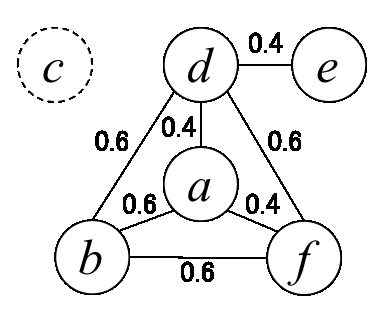
\includegraphics[scale=0.6]{./simg.eps}
\caption{表\ref{tbl:mt2g_out1}に対応する類似度グラフ。枝に示された数字は2つのアイテムの共起確率。\label{fig:mt2g_out1}}
\end{minipage}
\end{center}
\end{figure}


\subsection{書式}
\begin{verbatim}
書式) mtra2g.rb i= tid= item= [on=] eo= s= [sim=] [th=] [log=] [T=] [--help]

  ファイル名指定
  i=     : トランザクションデータファイル
  tid=   : トランザクションID項目名
  item=  : アイテム項目名
  on=    : 出力ファイル(節点)
  eo=    : 出力ファイル(辺:節点ペア)
  s=     : 最小支持度(全トランザクション数に対する割合による指定): 0以上1以下の実数】
  S=     : 最小支持度(トランザクション数による指定): 1以上の整数】
         : s=,S=共に指定しなければ、S=1が指定されたとして動作する。
  sim=   : 類似度
           R: resemblance
           P: normalized PMI
           省略時はs=もしくはS=の条件によってのみアイテム間に枝が張られる。
  th=    : sim=で指定された類似度について、ここで指定された値以上のアイテム間に枝を張る。
  log=   : パラメータの設定値をkey-value形式のCSVで保存するファイル名

  その他
  T= : ワークディレクトリ(default:/tmp)
  --help : ヘルプの表示
\end{verbatim}

\subsection{利用例}
\subsubsection*{Example 1: Basic Example}

Display similarity graph with 2 or more occurrence.
The example is shown above.


\begin{Verbatim}[baselinestretch=0.7,frame=single]
$ more dat1.csv
tid,item
T1,C
T1,E
T2,D
T2,E
T2,F
T3,A
T3,B
T3,D
T3,F
T4,B
T4,D
T4,F
T5,A
T5,B
T5,D
T5,E
T6,A
T6,B
T6,D
T6,E
T6,F
$ mtra2g.rb  S=2 tid=tid item=item i=dat1.csv oe=edge1.csv
#MSG# converting a named item into a numbered item ...
#MSG# run lcm enumerating 2 itemset ...
#MSG# creating the edge file ...
#END# /Users/stephane/.rvm/rubies/ruby-1.9.3-p448/bin/mtra2g.rb S=2 tid=tid item=item i=da
t1.csv oe=edge1.csv
$ more edge1.csv
node1,node2,support,void
A,B,0.5,
A,D,0.5,
A,E,0.3333333333,
A,F,0.3333333333,
B,D,0.6666666667,
E,B,0.3333333333,
E,D,0.5,
F,B,0.5,
F,D,0.6666666667,
F,E,0.3333333333,
\end{Verbatim}
\subsubsection*{Example 2: Add resemblance}

Based on example 1, add the degree of similarity criteria where resemblance is above 0.4.
By specifying \verb|on=|, only the frequency of appearance of item is returned as node information.


\begin{Verbatim}[baselinestretch=0.7,frame=single]
$ mtra2g.rb  S=2 sim=R th=0.4 tid=tid item=item i=dat1.csv oe=edge2.csv on=node2.csv
#MSG# converting a named item into a numbered item ...
#MSG# run lcm enumerating 2 itemset ...
#MSG# creating the edge file ...
#MSG# creating the node file ...
#END# /Users/stephane/.rvm/rubies/ruby-1.9.3-p448/bin/mtra2g.rb S=2 sim=R th=0.4 tid=tid i
tem=item i=dat1.csv oe=edge2.csv on=node2.csv
$ more node2.csv
node,support
A,0.5
B,0.6666666667
C,0.1666666667
D,0.8333333333
E,0.6666666667
F,0.6666666667
$ more edge2.csv
node1,node2,support,resemblance
A,B,0.5,0.75
A,D,0.5,0.6
A,E,0.3333333333,0.4
A,F,0.3333333333,0.4
B,D,0.6666666667,0.8
E,D,0.5,0.5
F,B,0.5,0.6
F,D,0.6666666667,0.8
\end{Verbatim}



